\chapter{Optimisation}

\section{Introduction}

The tests carried out during our load and stress testing were carried out on a server with an 'out of the box' configuration i.e. no changes were made to the default configuration. Similarly, the operating system was not optimised. In this section we aim to optimally configure the application for performance. 

We will specifically look at the following parameters:
\begin{itemize}
 \item Application server settings;
 \item Java Virtual Machine settings;
 \item Operating system settings;
\end{itemize}

When trying to optimise for performance we classify improvements by:
\begin{enumerate}
 \item Improving application performance for a constant load i.e. minimising response time for a given load and throughput;
 \item Maximising throughtput, keeping an acceptable response time i.e. increasing the number of users the application will support with an acceptable response\footnote{An extension to this improvement is to check for improved stress testing response.}
\end{enumerate}

We will focus on both aspects in optimising performance for AdaptiveCellsJ.

\section{Methodology}

In the optimisation process we will adhere to the following principles:
\begin{itemize}
 \item Only change one parameter at a time so as to isolate it;
 \item Carry out a a before and after test, measuring throughput, and response time on the client, and monitoring server parameters of CPU utilisation, network bandwidth utilisation, and JVM memory/heap utilisation (in tests involving memory);
 \item Ensure that the original load is high enough to adequetly stress the server (using monitoring tools and some adjustment as required);
 \item Allow the test to run for long enough to reach a steady state (at least ten minutes);
 \item Ensure uniformity for each test by restarting the application each time.
\end{itemize}

In testing we will follow the following general process:
\begin{enumerate}
 \item Carry out our base-line test on a pre-determined configuration i.e. with no changes from the defaults;
 \item Pick a client load that stresses the server adequetly - we will asses and adjust this by carrying out server monitoring;
 \item Carry out the optimisation and restart the application server;
 \item Carry out the test at the same client load as before the optimisation;
 \item Compare the throughput, and response time for the before and after configurations.
\end{enumerate}

\subsection*{Software and hardware environment}

We picked a test environment that had a powerful client machines, and a low specification server machine. This configuration was chosen so that client overloading would not occur.\footnote{As this would give erronous results.} During out tests the client machine was monitored and average CPU utilisation was well below 25\%. The client software, JMeter, was also monitored for heap usage, which also was well below the heap allocated (512MB).

We used JBOSS 4.0.4 (with JBOSS profiler installed), with Java 1.5.0 HotSpot. Client load was simulated with JMeter.v2.3.2.

\begin{figure}[ht]
 \centering
\begin{tabular}{| c | c | c |}
 \hline
  & \textbf{Client} & \textbf{Server} \\
 \hline
 \textbf{Operating system} & Open Suse 10.3 (64 bit) & Open Suse 10.3 (32 bit) \\
 \textbf{Memory} & 4GB & 1GB \\
 \textbf{Processor} & Intel Core 2 Duo (Quad core) @ 2.66 GHz & Intel P4 @ 2.8 GHz \\
 \hline
\end{tabular}
\caption{environment used}
\end{figure}

The network between the two machines was 100Mbit wired ethernet, using a ZyXEL P-660HW router.

\section{Optimisations}

\subsection*{Baseline Response}

To obtain a baseline measure of how this configuration responded under load we carried out some initial tests using the, 'out of the box', configuration. The first observation we made was that the default settings were possibly set too high for our hardware setup. Many authors recognise that setting parameters, such as thread pool sizes too high is a performance anti-pattern\cite{performance_solutions}. Initial monitoring indicated that the thread pool setting of 250 threads (for the embedded web container), was possibly too high. For the many of the parameters that are widely recognised to have the largest impact on performance require that the number of clients is larger than the thread pool\cite{model_server_settings_jee}. If this were not the case it would be very hard to measure as the top value of the parameter would have little to no impace. We found that at over 250 user the server processor utilisation was over 99\%. 

To find out the response of this setup we carried out the following test:
\begin{enumerate}
 \item Set the thread pool to 10, and the web container queue size to 40\footnote{carried out by editing values in server.xml file};
 \item Monitored the throughtput and response time for a range of clients;
 \item Observed with the point where throughput improvement started to fall off, and response time increased.
\end{enumerate}

Our JMeter test was structured so that we also tested fetching the initial static page (and embedded images), as well as submitting it. This was to ensure that we were testing all aspects of the application and stressing components of the JBOSS application server that the parameters may impact. We measured the total throughput i.e. the total number of served requests (number of times each web page element is served + number of submits of the page). We used config10 for this test as it is the most processor intensive of the configurations\footnote{see table in appendices}.
\newline

\begin{figure}[ht]
 \centering
 \scalebox{0.5}{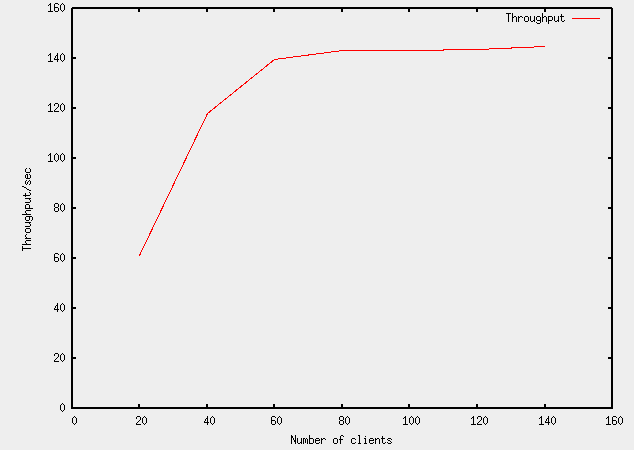
\includegraphics{Graphics/optimise_gen_response_tp.png}}
 \caption{Throughtput for a range of clients}
 \label{graph_response_tp}
\end{figure}

\begin{figure}[ht]
 \centering
 \scalebox{0.5}{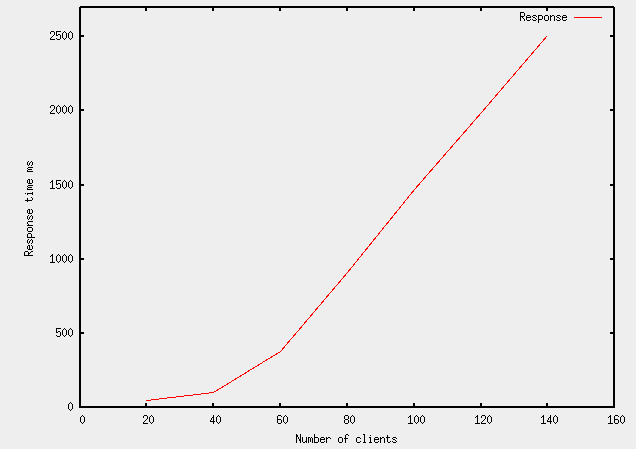
\includegraphics{Graphics/optimise_gen_response_rt.png}}
 \caption{Response time for a range of clients}
 \label{graph_response_rt}
\end{figure}

As the graphs in figures \ref{graph_response_tp} and \ref{graph_response_rt} show, we get a noticable drop in performance at 60 users. This is for the setting of 10 threads for the embedded web container, with a queue of 40. We will use this as a baseline figure. During our tests we measured server performance, CPU usage rose gradually as we increased the number of clients, but never rose above 90\%. Memory usage by the application was consistantly low. Both these indicate that this range of clients should give reliable, repeatable results and that we are not hitting hardware limits e.g. CPU, or memory. We will use this configuration as our baseline during the optimisation process.

\subsection*{Thread Pool Settings}

\subsubsection*{Embeded Web Container}

As identified in earlier the default settings for the embeded web container are two high for our environment. This results in maxing out the CPU as we increase the number of clients. For the purpose of establishing our base line configuration we greatly reduced our the number of threads and the queue size for the embeded web container (EWC), to 10 threads and a queue of 40 requests. Other work has been done into how these two parameters impact performance\cite{model_server_settings_jee}, concluding that these parameters significantly impact performance. During the baseline tests we monitored the counter 'currentThreadsBusy', provided by the JMX bean jboss.web. We observed that this parameter quickly rose to 10, indicating that all 10 threads in the pool were working. Articles indicate that the number of threads used should be less than 70\%-80\% of the maxThreads value (in our case 10)\cite{master_the_boss}. 

We will investigate the effect of increasing the thread pool size and the queue size. In our baseline tests we did not receive any request timeout responses. We should have received this error if a request arrived when the queue was full. This theory was backed up by our test. We increased the queue size by from 40 to 100, which made little to no difference to our results (less than 1\% deviation from the baseline measure). For a thread pool of 10 this queue size would seem to be sufficient.

Moving on to investigate the effect of increasing the web container threadpool setting. Using the guideline above we picked a thread pool size of 100 threads, if the processor did not max out when the currentBusyThreads values was close to 100, we would increase this. We re-ran the baseline tests, but with the thread pool set to 100.

\begin{figure}[ht]
 \centering
 \scalebox{0.5}{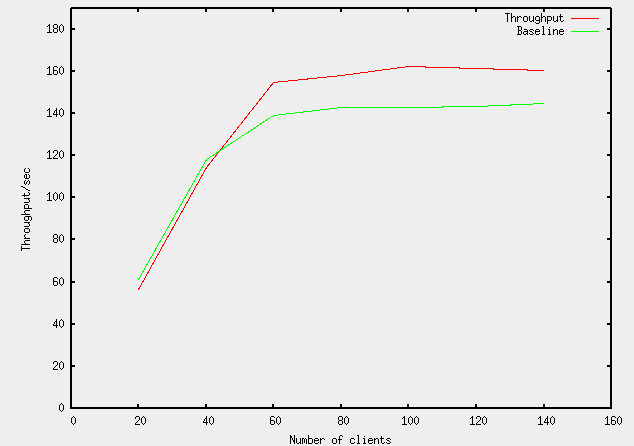
\includegraphics{Graphics/wc_throughput_thread_pool_tp.png}}
 \caption{Throughput baseline compared to larger thread pool.}
 \label{graph_tp_tput}
\end{figure}

\begin{figure}[ht]
 \centering
 \scalebox{0.5}{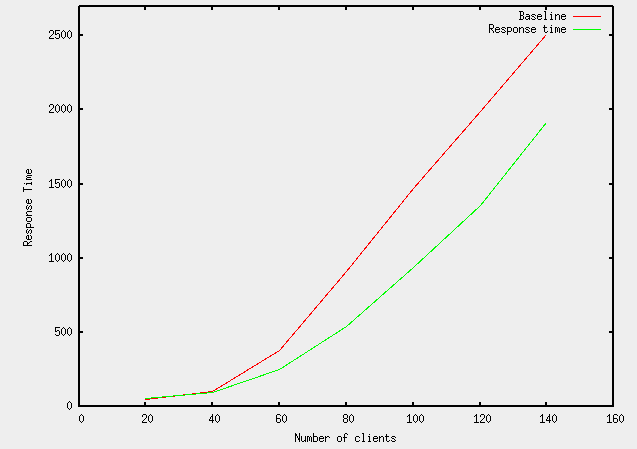
\includegraphics{Graphics/wc_response_thread_pool_tp1.png}}
 \caption{Response time, baseline compared to larger thread pool.}
 \label{graph_tp_rt}
\end{figure}

As the graphs in figures \ref{graph_tp_tput}, and \ref{graph_tp_rt} indicate, performance did improve with the new thread pool setting. Both throughput and response time showed improvements. Comparing the throughput to the baseline response, we see that the drop off occurs later (at 60 clients, compared to 40 clients), giving a ceiling that is higher by approximately 20 requests/second. We noted that at around 120 clients the the server processor was operating at nearly 100\%, indicating that we were at saturation of this resource and that this is probably a hardware limit. Maximum throughput would be governed, in this case, by the CPU resouce, and is given by 1/S (mean service time) \cite{model_server_settings_jee}\cite{performance_solutions}. In our case the system would be modelled by a closed queueing network model\footnote{this will be discussed more fully in the modelling section.}, for this model the arrival rate is state dependent as if we have K clients, but there are k jobs at the server (waiting for service) then there are only K-k clients that can send in new requests\cite{model_server_settings_jee}. If the system is using all the threads in the web container, then any new requests will be queued (i.e. giving a bigger queue). This means that k will be higher in our baseline case, than for a system with more threads in the pool. As \begin{math}\lambda_{k} \propto (K-k)\end{math} - where \begin{math}\lambda_{k}\end{math} is arrival rate for kth request\cite{model_server_settings_jee}, then this would explain our higher throughput.

The results for response time also showed significant improvement, we note that up to 120 clients the improvement increased with number of clients (at which point we reached CPU saturation). This also makes sense as response time = queue residence time + service time, increasing the number of threads would decrease the queue residence time, and hence decrease response time. 

This test would show that a value of around 100 threads, and a queue size of 40 is sufficient optimisation to improve performance up to around 120 clients. Above this demand we seem to be hitting processor saturation.

\subsubsection*{JBOSS Thread Pool}

Once the embeded web container has dealt with the request it must be passed onto the EJB tier. As shown in figure \ref{fig_bean_calling}, this tier calls a number of beans (depening on the configuration). These requests are carried out by a thread pool, in which the queue size and number of threads is configurable in a similar manner to the embedded web container. The parameters are specified in the file jboss-service.xml. We left the queue size at the default of 1,000 and altered the MaxPoolSize parameter (default is 10 threads). During our tests we monitored the queueSize measure in the jboss.system JMX bean, the guideline\cite{master_the_boss} is that if the queueSize approaches the MaxThreadPool size then you may need more threads (if the system is not at CPU/Memory saturation). We kept the number of clients at 60, and we used the configuration in set for the web container (100 threads, queue of 40), rather than the base line configuration. This was chosen because we wanted to avoid CPU saturation, hence the 60 clients, but balanced against this we wanted to maximise the rate that requests reached the EJB tier. Through trial and error we established that a load level of 60 clients provided adequete load without saturation.

We ran our test, with different numbers for MaxThreadPool (1, 5, 10, 15, 20, 25). We encoutered some unusual results. Firstly the queueSize was always 0, except for the case of having 1 thread in the pool, in which case the queueSize was always 1. This seems unusual, and unexplainable at the moment. Secondly changing the MaximumPoolSize parameter had no effect on throughput or response times (less than 4\% deviation). We tried changing other parameters (e.g. BlockingMode), but this made no difference. Further investigation would be required to understand what was happening here. For the queue length to be 1 then by Little's law RT = (1/throughput) - we will investigate this in the modelling section.

\subsection*{Garbage Collection and Memory Usage}

We monitored the JVM heap usage and garbage collection by using the -xloggc flag. The resulting log file was analysed with gcviewer. We observed the results indicated below (before row). The throughput was already quite good, at 99.34\%, but the application pauses was perhaps a little poor at 4.05s. We increased the heapsize, setting the minimum and maximum to the same value of 512m. We also changed the heap ratio, giving the young generation 25\% of the heap. This was done because for this application we know that the beans are stateless and that each bean frees up it's memory allocated fairly soon. This was also shown to be true by looking at the graph of heap usage, the application allocates it's memory and frees it shortly afterwards. The trace also backed this up by showing only 10\% of the tenured generation was used, but 50\% of the young generation was used.

As shown in figure \ref{gc_performance} we made a small improvement in throughput, and a large improvement in pauses (owing to fewer garbage collections). This performance seemed adequate, and confirms our theory that garbage collection is not a big factor for this application, even with the default settings.

\begin{figure}[h]
 \centering
\begin{tabular}{| c | c | c |}
 \hline
  & Throughput & Acc pauses\\
 \hline
 Before change & 99.34\% & 4.05s \\
 After change 5 & 99.75\% & 1.3s \\
 \hline
\end{tabular}
 \caption{Garbage collection performance}
 \label{gc_performance}
\end{figure}

\subsection*{Other possible areas for optimisation}

After analysing results from our load and stress testing, and also the results of the optimisations. We observed that for this appliction after optimisation, the biggest bottle neck is CPU saturation. 

There are a number of other areas we could optimise (given the time), but we feel that these areas would produce diminishing returns. The areas are:

\begin{itemize}
 \item Operating system settings (network settings, memory);
 \item Slim down JBOSS (set production settings e.g. turn of JSP compilation, remove surplus services e.g. mail, log4j);
 \item Tune pool size (we know that our beans are stateless session beans, we could look at the object pool size).
\end{itemize}

\section{Summary}

Our optimisations have given a significant improvement in throughput and response time, within the capacity of our test environment. 
